\section{Sample Use Case}

To demonstrate the power of the \textit{Reagent} system, we demonstrate it within a 
toy domain of analyzing football teams within the premier league team and building 
an ontology in OWL~\cite{staab_web_2004} around it. The system starts with no knowledge within the ontology
and the goal is at the end to have built up a minimal relationship graph of the couple of 
entities we encounter as well as their properties, as automatically as possible.
To accomplish this, we utilize content from the websites ESPN and SkySports. The
output of the UI that is displayed to the user is shown in the following figures.
Within the figures, the top left contains the current site/table being
inspected. Underneath that, there is a display to show the current state of the ontology as it 
is being built, shown using WebVOWL~\cite{lambrix_webvowl:_2015}. On the right is the
running transcript of the system with queries from the user being prefixed with a yellow 
``Person'' and the system's responses being prefixed with a blue ``Watson''. 

%\begin{figure}
%\centering
%\includegraphics[width=0.45\textwidth]{figures/skysports_premier.png}
%\caption{Premier League Table from SkySports.}
%\label{fig:skysports_premier}
%\end{figure}

\begin{figure*}[hbtp]
\centering
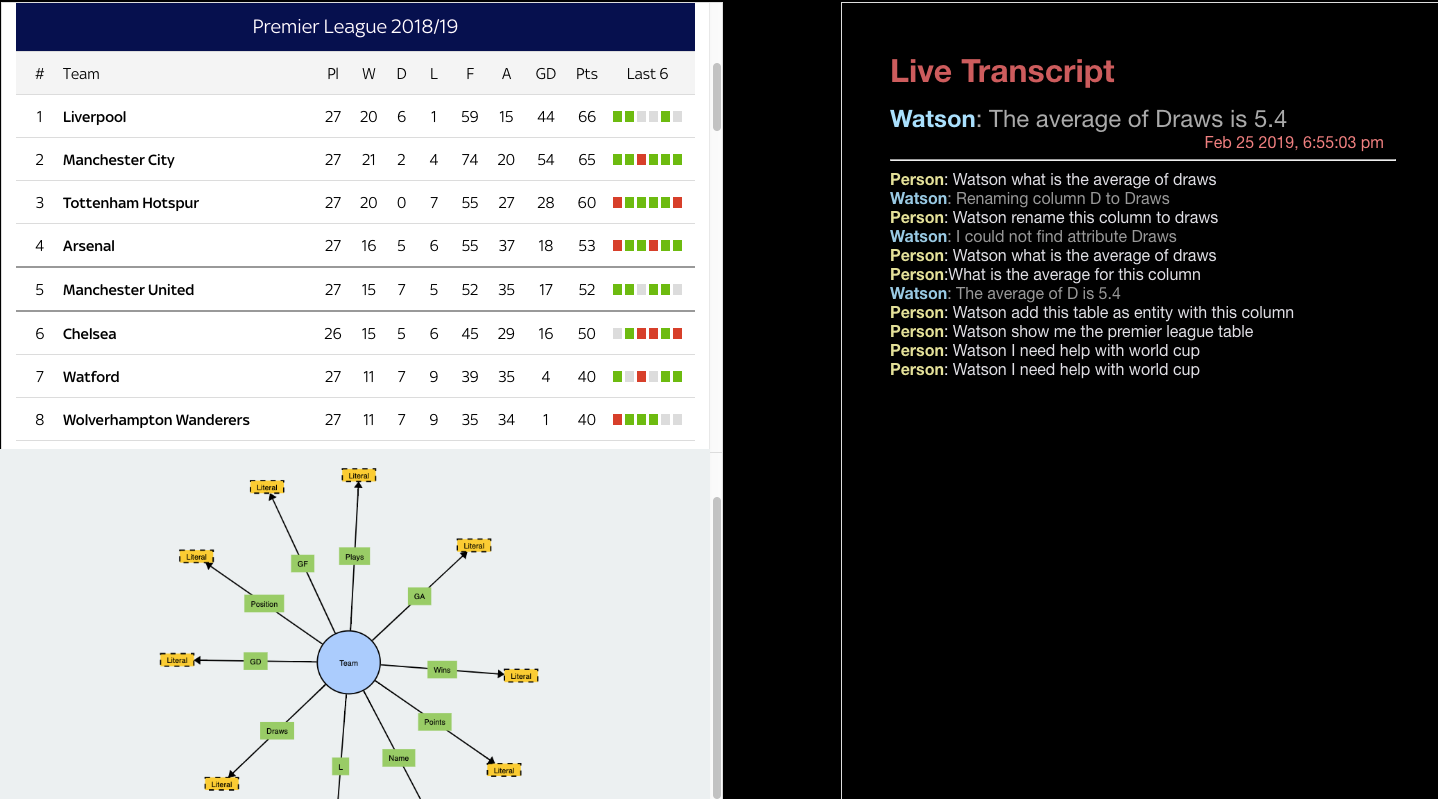
\includegraphics[width=0.8\textwidth]{chapters/03_reagent/figures/use_case_1.png}
\caption{Display of system after adding Team entity.}
\label{fig:reagent_use_case_1}
\end{figure*}

To start with, we open a page from SkySports that shows the current standings
of all teams in the football premier league~\cite{skysports_table}. To begin building
our ontology, the user can point at the displayed table and then state ``Add this table
as entity {\em team}'' or alternatively point at the column marked ``Team'' and say ``Add this
table as entity using this column''. The executor will contact \textit{Reagent} to get the columns
of the table under question. From there, the executor will send the list of columns, as well
as the entity name to our ontology as a simple JSON object, which in then converted by an
ontology pipeline into the appropriate OWL RDF structure to be stored, marking the entity as a 
Class and the columns as Object Properties linked to the class, and pointing at concrete 
Literals. After this step is completed, all entries in the table are then saved as instances
for that Class, ready to be queried. Additionally, anytime a user comes back to this page,
or a page that has a table of nearly identical structure, the system will automatically infer that the table
is of the Team class, along with automatically transforming any abbreviated columns to known
attributes if possible. Either before or after adding an entity to the ontology, a user can always go and
fill in the gaps as necessary in the system's understanding of the columns. For example, in the case of 
SkySports, while the first 4 columns have a title tag (displayed when hovering over the abbreviation), 
the rest do not and so the system saves them only as abbreviations (e.g. ``D'', ``L'', etc.). 
Additionally, while we can query the system for values of the fully named attributes, we cannot at this
time get anything for the abbreviations for what they stand for. For example, if the user
tries to ask ``What is the average of draws'', the system will respond with 
``I could not find the attribute draws''. To remedy this, the user can point at one of these
columns and then issue a new name for the column. For example, to update the
label marked ``D'', the user would point at the column and say ``Rename this column
name to Draws'', which gets automatically mirrored to our
ontology. Following this, the user can then repeat a request for the
average of draws and the system will now successfully respond with ``The average of Draws is 5.4''. The result of this sequence is shown in Figure~\ref{fig:reagent_use_case_1}, wherein we still have several more attributes that
have to be renamed due to lacking the title tag, using a similar command as
above.

After being satisfied with the constructed ``Team'' entity, the user may want
to then look at the players of one of these teams. To
do this, we open a page of a team (e.g. Manchester United) from ESPN~\cite{espn_squad_table}. When we open
the page, the system scans the table, sees if the table matches
any saved entity, which is just ``Team'' at this time and as the columns does not match the ``Team'' entity's attributes,
the system states ``I do not recognize this entity. Please add it''. Similar
to the previous entity, the user
can save the table as a new entity by first pointing at it and then saying ``Add this table as entity 'player''', which
adds a new entity ``Player'' to our ontology along with all of the columns in the
table in the same process as before. A new Player entity then appears
alongside the Team entity in the Ontology Viewer of the display, which
is shown in Figure~\ref{fig:reagent_use_case_2}.

In this case, all of the terms have title tags and so are all properly labeled when they were added, so the user does not have to do any further renaming. The user can
now query the system about these saved attributes, such as pointing at the first
row in the table and asking ``How many appearances does the player have'' which
the system responds with ``The player has 24 appearances''.

\begin{figure*}[hbtp]
\centering
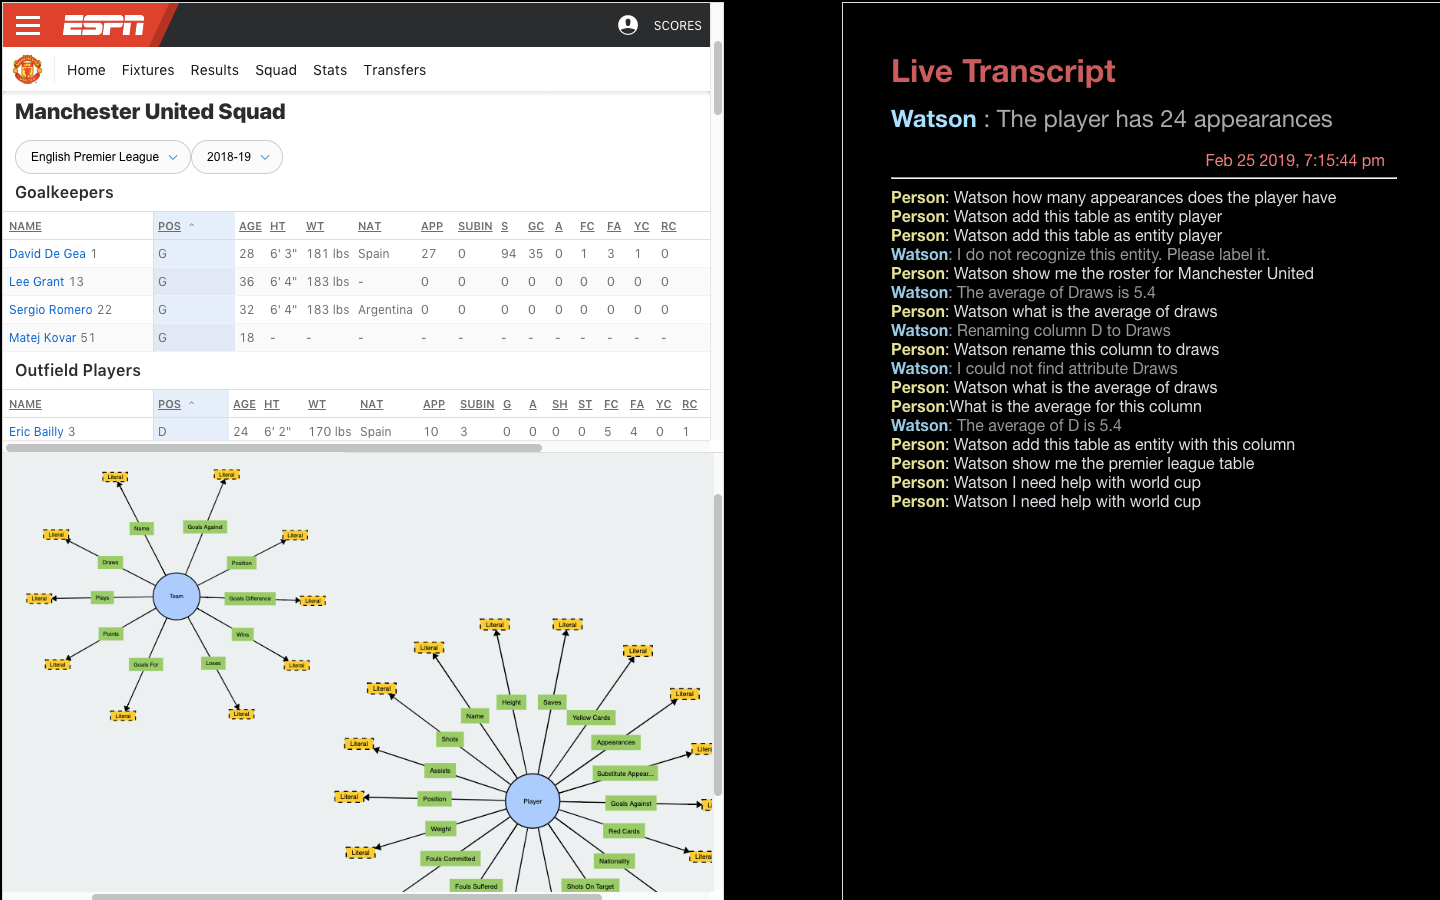
\includegraphics[width=0.8\textwidth]{chapters/03_reagent/figures/use_case_2.png}
\caption{Display of system after adding the Player entity.}
\label{fig:reagent_use_case_2}
\end{figure*}

To complete our basic ontology, the user can now add a relationship
between the two saved entities. To do this, the user can simply issue
the query ``Add relationship part of between entity team and player''. The
system then adds a new Object Property link between the two marked as 
``partOf'', as shown in Figure~\ref{fig:reagent_use_case_3}. Through this connection,
the user can now start issuing queries that utilize information from both of the opened tables. For example,
the user can ask ``How many wins does the team of this player have?'' while pointing
at the player table. The system will look up who that player's team is, cross-reference it
back to the prior table, and extract the requested information, outputting it to the user.

\begin{figure*}[hbtp]
\centering
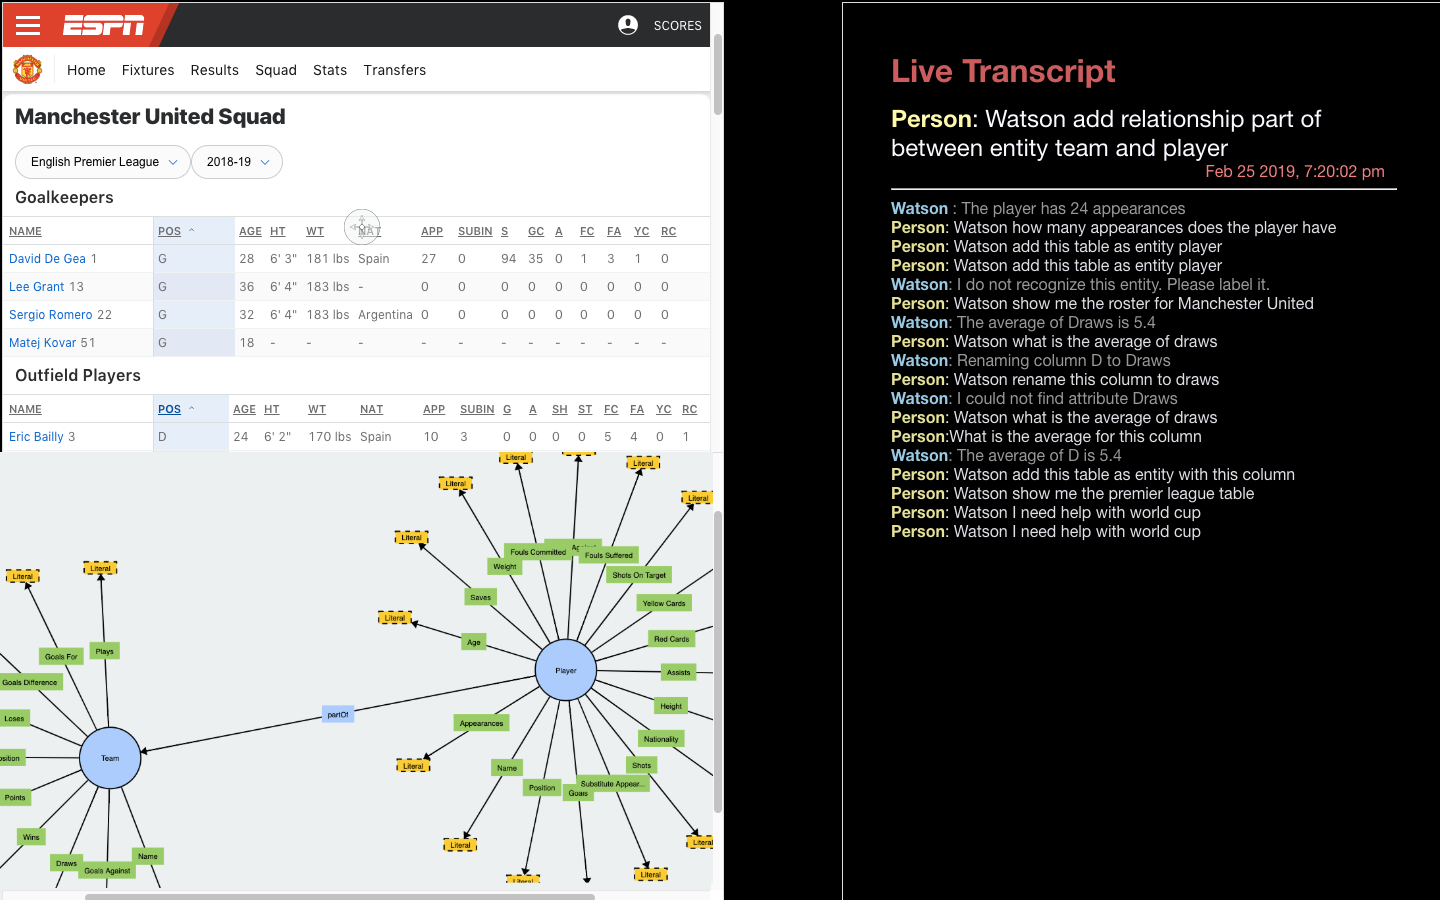
\includegraphics[width=0.8\textwidth]{chapters/03_reagent/figures/use_case_3.png}
\caption{Display of the system with the final ontology.}
\label{fig:reagent_use_case_3}
\end{figure*}

After building this ontology, whenever a user goes to a page that contains
similar content, the system will, as before, attempt to determine if the
content is of a known entity based on the table's columns, even if
the table has more or fewer attributes than have been seen. If a table is seen
with more attributes than saved in our ontology, it will ask the user if they
wish to add the attributes to the saved entity.
